\documentclass[12pt,oneside,a4paper,parskip]{scrbook}
\usepackage[utf8]{inputenc}
\usepackage{csquotes}
\usepackage[ngerman]{babel}
\usepackage{floatflt}
\usepackage{subfigure}
\usepackage[pdftex]{graphicx}
\usepackage[hidelinks]{hyperref}
\usepackage{color}
\usepackage{amssymb}
\usepackage{textcomp}
\usepackage{nicefrac}
\usepackage{scrhack}
\usepackage{pdfpages}
\usepackage{float}
\usepackage{pdflscape}
\usepackage{subfigure}
\usepackage{pdfpages}
\usepackage[verbose]{placeins}
\usepackage[nouppercase,headsepline,plainfootsepline]{scrpage2}
\usepackage{listings}
\usepackage{xcolor}
\usepackage{color}
\usepackage{caption}
\usepackage{subfigure}
\usepackage{epstopdf}
\usepackage{longtable}
\usepackage{setspace}
\usepackage{booktabs}
\usepackage{hyperref}
\usepackage{enumitem}
\usepackage[style=numeric,backend=bibtex]{biblatex}
\bibliography{literatur}


%%%%%%%%%%%%%%%%%%%
%% definitions
%%%%%%%%%%%%%%%%%%%
\def\BaAuthor{René Ziegler}
\def\BaTitle{Über die Automatisierung der Entwicklung von Software Generatoren}
\def\BaSupervisorOne{Prof.\ Dr.\ Peter Braun}
\def\BaSupervisorTwo{M.Sc. Tobias Fertig}
\def\BaDeadline{\today}

\hypersetup{
pdfauthor={\BaAuthor},
pdftitle={\BaTitle},
pdfsubject={Subject},
pdfkeywords={Keywords}
}

%%%%%%%%%%%%%%%%%%%
%% configs to include
%%%%%%%%%%%%%%%%%%%
\colorlet{punct}{red!60!black}
\definecolor{background}{HTML}{EEEEEE}
\definecolor{delim}{RGB}{20,105,176}
\colorlet{numb}{magenta!60!black}

\definecolor{gray}{rgb}{0.4,0.4,0.4}
\definecolor{darkblue}{rgb}{0.0,0.0,0.6}
\definecolor{cyan}{rgb}{0.0,0.6,0.6}

\definecolor{pblue}{rgb}{0.13,0.13,1}
\definecolor{pgreen}{rgb}{0,0.5,0}
\definecolor{pred}{rgb}{0.9,0,0}
\definecolor{pgrey}{rgb}{0.46,0.45,0.48}

\lstset{
  basicstyle=\ttfamily,
  columns=fullflexible,
  showstringspaces=false,
  commentstyle=\color{gray}\upshape
  linewidth=\textwidth
}

\lstdefinelanguage{json}{
    basicstyle=\normalfont\ttfamily,
    numbers=left,
    numberstyle=\scriptsize,
    stepnumber=1,
    numbersep=8pt,
    showstringspaces=false,
    breaklines=true,
    backgroundcolor=\color{background},
    literate=
     *{0}{{{\color{numb}0}}}{1}
      {1}{{{\color{numb}1}}}{1}
      {2}{{{\color{numb}2}}}{1}
      {3}{{{\color{numb}3}}}{1}
      {4}{{{\color{numb}4}}}{1}
      {5}{{{\color{numb}5}}}{1}
      {6}{{{\color{numb}6}}}{1}
      {7}{{{\color{numb}7}}}{1}
      {8}{{{\color{numb}8}}}{1}
      {9}{{{\color{numb}9}}}{1}
      {:}{{{\color{punct}{:}}}}{1}
      {,}{{{\color{punct}{,}}}}{1}
      {\{}{{{\color{delim}{\{}}}}{1}
      {\}}{{{\color{delim}{\}}}}}{1}
      {[}{{{\color{delim}{[}}}}{1}
      {]}{{{\color{delim}{]}}}}{1},
}

\lstset{language=xml,
  morestring=[b]",
  morestring=[s]{>}{<},
  morecomment=[s]{<?}{?>},
  stringstyle=\color{black},
  numbers=left,
  numberstyle=\scriptsize,
  stepnumber=1,
  numbersep=8pt,
  identifierstyle=\color{darkblue},
  keywordstyle=\color{cyan},
  backgroundcolor=\color{background},
  morekeywords={xmlns,version,type}% list your attributes here
}

\lstset{language=Java,
  showspaces=false,
  showtabs=false,
  tabsize=4,
  breaklines=true,
  keepspaces=true,
  numbers=left,
  numberstyle=\scriptsize,
  stepnumber=1,
  numbersep=8pt,
  showstringspaces=false,
  breakatwhitespace=true,
  commentstyle=\color{pgreen},
  keywordstyle=\color{pblue},
  stringstyle=\color{pred},
  basicstyle=\ttfamily,
  backgroundcolor=\color{background},
%  moredelim=[il][\textcolor{pgrey}]{$$},
%  moredelim=[is][\textcolor{pgrey}]{\%\%}{\%\%}
}


%%%%%%%%%%%%%%%%%%%
%% custom config
%%%%%%%%%%%%%%%%%%%
\setcounter{secnumdepth}{3}
\setcounter{tocdepth}{3}
\begin{document}


%%%%%%%%%%%%%%%%%%%
%% Titelseite
%%%%%%%%%%%%%%%%%%%


\frontmatter
\titlehead{%  {\centering Seitenkopf}
  {Hochschule für angewandte Wissenschaften Würzburg-Schweinfurt\\
   Fakultät Informatik und Wirtschaftsinformatik}}
\subject{Bachelorarbeit}
\title{\BaTitle\\[15mm]}
\subtitle{\normalsize{vorgelegt an der Hochschule f\"{u}r angewandte Wissenschaften W\"{u}rzburg-Schweinfurt in der Fakult\"{a}t Informatik und Wirtschaftsinformatik zum Abschluss eines Studiums im Studiengang Informatik}}
\author{\BaAuthor}
\date{\normalsize{Eingereicht am: \BaDeadline}}
\publishers{
  \normalsize{Erstpr\"{u}fer: \BaSupervisorOne}\\
  \normalsize{Zweitpr\"{u}fer: \BaSupervisorTwo}\\
}

%\uppertitleback{ }
%\lowertitleback{ }

\maketitle


%%%%%%%%%%%%%%%%%%%
%% abstract
%%%%%%%%%%%%%%%%%%%

\section*{Zusammenfassung}

TODO

\section*{Abstract}

TODO

\newpage
\chapter*{Danksagung}



%%%%%%%%%%%%%%%%%%%
%% Inhaltsverzeichnis
%%%%%%%%%%%%%%%%%%%
\tableofcontents



%%%%%%%%%%%%%%%%%%%
%% Main part of the thesis
%%%%%%%%%%%%%%%%%%%
\mainmatter


\chapter{Einführung}\label{ch:intro}

Als Henry Ford 1913 die Produktion des Modell T, umgangssprachlich auch Tin Lizzie genannt, auf Fließbandfertigung umstellte, revolutionierte er die Automobilindustrie. Ford war nicht der erste, der diese Form der Automatisierung verwendete. Bereits 1830 kam in den Schlachthöfen von Chicago eine Maschine zum Einsatz, die an Fleischerhaken aufgehängte Tierkörper durch die Schlachterei transportierte. Bei der Produktion des Oldsmobile Curved Dash lies Ranson Eli Olds 1910 erstmals die verschiedenen Arbeitsschritte an unterschiedlichen Arbeitsstationen durchführen. Fords Revolution war die Kombination beider Ideen. Er entwickelte eine Produktionsstraße, auf welcher die Karossen auf einem Fließband von Arbeitsstation zu Arbeitsstation befördert wurden. An jeder Haltestelle wurden nur wenige Handgriffe von spezialisierten Arbeitern durchgeführt \cite{sagerso2008}.

Fords Vision war es, ein Auto herzustellen, welches sich Menschen aller Gesellschaftsschichten leisten konnten. Durch die Reduktion der Produktionszeit der Tin Lizzie von 12,5 Stunden auf etwa 6 Stunden konnte Ford den Preis senken. Kostete ein Auto des Model T vor der Einführung der Produktionsstraße 825\$, erreichte der Preis in den Jahren danach einen Tiefststand von 259\$ \cite{reichlesz2010}. Setzt man diesen Preis in ein Verhältnis mit dem durchschnittlichen Einkommen in den USA, das 1910 bei jährlich 438\$ lag, kann man sagen, dass Fords Traum durch die eingesetzten Techniken Realität wurde \cite{usembassyodnumbers}.

Im Zuge der weiteren Entwicklung der Robotik wurden immer mehr Aufgaben, die bisher von Menschen am Fließband durchgeführt wurden, von Automaten übernommen. In der Automobil-Industrie war General Motors der erste Hersteller, bei welchem die Produktionsstraßen im Jahr 1961 mit 66 Robotern des Typs Unimation ausgestattet wurden. Bis zur Erfindung des integrierten Schaltkreises in den 1970ern waren die Roboter ineffizient. Der Markt für industrielle Roboter explodierte jedoch in den Folgejahren. Im Jahr 1984 waren weltweit ungefähr 100.000 Roboter im Einsatz \cite{czaeis2000, wallen2008}.

Die industrielle Revolution prägte die Autoindustrie: von der Erfindung auswechselbarer Teile 1910 bei Ransom Olds, über die Weiterentwicklung des Konzepts unter der Verwendung von Fließbändern bei Ford im Jahr 1913, bis hin zur abschließenden Automatisierung mit Industriellen Robotern in den frühen 1980ern \cite{czaeis2000}.

\section{Motivation}

\begin{quote}
	\glqq If you can compose components manually, you can also automate this process.\grqq
\end{quote}

Das hervorgehobene Zitat nennen Czarnecki und Eisenecker die Automation Assumption. Diese allgemein gehaltene Aussage lässt die Parallelen, die die beiden Autoren zwischen der Automatisierung der Automobilindustrie und der automatischen Code Generierung sehen, erkennen. Dafür müssten die einzelnen Komponenten einer Softwarefamilie derart gestaltet werden, dass diese austauschbar in eine gemeinsame Struktur integriert werden können. Des weiteren müsste klar definiert sein, welche Teile eines Programms konfigurierbar seien und welche der einzelnen Komponenten in welcher Konfiguration benötigt werden. Setzt man dieses definierte Wissen in Programmcode um, könnte ein solches Programm eine Software in einer entsprechenden Konfiguration generieren \cite{czaeis2000}.

Konkret bedeutet dies, dass entweder eine vorhandene Implementierung in Komponenten zerlegt werden muss oder eine für die Zwecke der Codegenerierung vorgesehene Referenzimplementierung geschrieben wird. Codeabschnitte, die in Ihrer Struktur gleich sind, sich jedoch inhaltlich unterscheiden, müssen formal beschrieben werden \cite{stahl2007}. Ein solches abstraktes Modell wird dann mit Daten befüllt. Schlussendlich wird ein Generator implementiert, der den Quellcode für unterschiedliche Ausprägungen eines Programms einer Software-Familie, auf Basis des konkreten Modells, generieren kann \cite{fowler2010}.

Sowohl bei der Umsetzung von einzigartigen Anwendungen, als auch bei der Verwirklichung von Software mit mehreren Varianten, kann die Verwendung von bereits verfügbaren Code Generatoren oder die Entwicklung eigener Code Generatoren vorteilhaft sein. Die Entwicklungsgeschwindigkeit könnte erhöht, die Softwarequalität gesteigert und Komplexität durch Abstraktion reduziert werden \cite{stahl2007}. Allgemein wird weniger Zeit benötigt, um eine größere Vielfalt an ähnlichen Programmen zu entwickeln \cite{czaeis2000}.

Bisher müssen fast alle Teilaufgaben bei der Umsetzung eines Code Generators manuell durchgeführt werden. Werkzeuge wie Language Workbenches können Code bis zu einem gewissen Grad automatisiert generieren oder interpretieren. Sie haben aber in erster Linie die Aufgabe, den Entwickler beim Design von externen domänenspezifischen Sprachen zu unterstützen und dienen als Entwicklungsumgebung für die Arbeit mit der Sprache \cite{fowler2010}.

Soll ein Projekt Modellgetrieben entwickelt werden, so lohnt sich dies wirtschaftlich gesehen erst, wenn auf Basis des entwickelten Modells mehrere Programme entwickelt wurden \cite{}. Einer der Teilschritte dieses Entwicklungsprozesses ist die Planung und Implementation des Code Generators. Durch ihre hohe Komplexität, ist diese Aufgabe sehr zeitaufwendig \cite{}.

ÜBERARBEITEN
\section{Zielsetzung}

In dieser Arbeit soll untersucht werden, ob und wie die Entwicklung eines Codegenerators automatisiert werden kann. Eine zusätzliche Ebene der Indirektion könnte das komplexe Thema der Modellgetriebenen Softwareentwicklung weiter vereinfachen und somit Code Generierung für mehr Entwickler zugänglicher und somit auch wirtschaftlicher machen.

Im speziellen wird analysiert, wie ein Meta-Generator zur Erhöhung der Wirtschaftlichkeit modellgetriebener Softwareentwicklung umgesetzt werden könnte. Zu diesem Zweck wird eine beispielhafte Java Anwendung erarbeitet, welche es ermöglichen soll, vorhandenen Java Quelltext so mit Informationen anzureichern, dass aus diesem ein Meta-Generator abgeleitet werden kann.

\section{Aufbau der Arbeit}

Die sieben Kapitel dieser Bachelorarbeit versuchen den Leser Stück für Stück an das komplexe Thema der Meta-Generierung heranzuführen. Da es nicht möglich ist im Rahmen einer vergleichsweise kurzen Thesis wie dieser sämtliche Grundlagen der Informatik zu beschreiben, wird ein solides Fundament aus Vorwissen, wie man es zum Beispiel in einem Bachelorstudium erwerben kann, vorausgesetzt.

Eingeleitet wird diese Arbeit mit einem Kapitel zur Motivation und Zielsetzung, in welchem aufgezeigt werden soll warum es sinnvoll ist, sich mit dem Thema der modellgetriebene Softwareentwicklung zu beschäftigen. 

Das zweite Kapitel behandelt die erweiterten, grundlegenden Kenntnisse, die zum Verständnis des Textes notwendig sind. Hier wird sowohl auf die modellgetriebene Softwareentwicklung, als auch auf die Software Architektur und die Verwendung von Design Pattern objektorientierter Programmierung eingegangen.

Aufbauend auf dem vorhergehenden Abschnitt sollte das dritte Kapitel, die Analyse, gut verständlich sein. Hier wird zuerst der wirtschaftliche Aufwand konventioneller Softwareprojekte mit dem Aufwand von Projekten welche ein modellgetriebenen Ansatz verfolgen verglichen. Danach werden die Probleme der einzelnen Teilschritte bei der Automatisierung der Entwicklung des Codegenerators untersucht.

Das Konzept Kapitel erläutert nun den im Proof-of-Concept verfolgten Lösungsansatz der analysierten Probleme. Zur Veranschaulichung kommen hier lediglich Diagramme zum Einsatz, dadurch sollte es möglich sein die allgemeine Idee hinter der Implementation leichter zu verstehen und den Ansatz losgelöst von der Umsetzung weiter zu verfolgen.

Im fünften Kapitel werden jetzt zum einen die verwendeten externen Bibliotheken kurz vorgestellt, zum anderen wird genau auf die Architektur der entwickelten Anwendung eingegangen. Die Funktionsweise und der Aufbau jeder Programmkomponente wird anhand von Quelltext Auszügen genau erläutert, mithilfe von Beispielen wird die Verwendung der einzelnen Einheiten demonstriert.

Das vorletzte Kapitel der Arbeit evaluiert sowohl das Konzept als auch die Umsetzung aller Module im Detail. Außerdem wird die allgemeine Softwarequalität des entwickelten Generators nach bewährten Kriterien untersucht. Besonders umfangreich werden die Grenzen des Lösungsansatzes diskutiert und mögliche Antworten auf die hieraus entstehenden Fragen angesprochen.

Mit dem siebten Kapitel werden Inhalt und Erkenntnisse der Arbeit noch einmal in gebündelter Form zur Verfügung gestellt. Ein ausführlicher Ausblick soll die vielen möglichen Anknüpfungspunkte dieser Thesis aufzeigen.

\chapter{Grundlagen}

Um die grundlegenden Zusammenhänge zu verstehen wird im folgenden auf die verschiedenen Aspekte und Teilschritte der modellgetriebenen Softwareentwicklung eingegangen. Begriffe und Konzepte die in der Arbeit zur Anwendung kommen, werden eingeführt und definiert. Danach wird auf einige Grundlagen der Softwarearchitektur, vor allem auf die Prinzipien der Softwaretechnik eingegangen. Da in der Implementation auf einige Design Pattern objektorientierter Programmierung zurückgegriffen wird, werden deren Zweck, Aufbau und Anwendbarkeit abschließend in diesem Kapitel erläutert.

\section{Modellgetriebene Softwareentwicklung (MDSD)}

\begin{quote}\glqq Modellgetriebene Softwareentwicklung (Model Driven Software Development, MDSD) ist ein Oberbegriff für Techniken, die aus formalen Modellen automatisiert lauffähige Software erzeugen.\grqq \end{quote}

Die obige Definition stammt aus dem Buch modellgetriebene Softwareentwicklung von Thomas Stahl und Markus Völter \cite[S. 11]{stahl2007}. Sie lässt sich gut erläutern wenn man sie in drei Teile zerlegt.

Zunächst einmal wäre dort der Ausdruck "formales Modell". Damit ist ein Modell gemeint welches einen Teil einer Software vollständig beschreibt. Jedoch soll das nicht heißen, dass dieses Modell allumfassend ist, sondern was genau von diesem Modell beschrieben wird muss eindeutig reguliert sein \cite[S. 11f.]{stahl2007}. Weiterhin bezieht sich die Definition darauf dass lauffähige Software erzeugt wird. D. h. wird das formale Modell nur zur Dokumentation verwendet oder dient es als Information zur händischen Umsetzung, so kann man das laut Stahl und Völter nicht als modellgetriebene Softwareentwicklung bezeichnen \cite[S. 12]{stahl2007}. Der letzte Teil der Definition den die Autoren explizit erläutern ist, dass die Umwandlung von Modell zu ausführbar Software automatisiert erfolgen soll. Insbesondere soll der Quelltext nicht nur einmal generiert und dann manuell verändert und weiterentwickelt werden, sondern das Modell soll anstelle des Quelltextes treten. Der Quelltext wird aus den geänderten Modellen generiert, dadurch kann aktueller und einheitlicher Quellcode gewährleistet werden \cite[S. 13]{stahl2007}.

In der Literatur findet sich auch die alternative Bezeichnung Model Driven Development (MDD) \cite{selic2003,atkinson2003}. Diese Thesis wird jedoch durchgängig die Bezeichnung MDSD verwenden.

Auch der Model Driven Architecture (MDA) Ansatz der Object Management Group (OMG) beschäftigt sich mit modellgetriebener Softwareentwicklung \cite{mdaguide}. Dieser Ansatz beschreibt detailliert und umfassend den Gesamtprozess von der Analyse bis hin zur Implementation und führt eigene Standards ein. 

Czarnecki und Eisenecker verwenden den Ausdruck Generative Programming, definieren ihn jedoch in den wesentlichen Punkten vergleichbar zu MDSD. Wobei Generative Programming nach Czarnecki und Eisenecker nach vollständiger Automation strebt und ein vollständiges Zwischen- oder Endprodukt erzeugen soll \cite[S. 5]{czaeis2000}. Für MDSD merken Stahl und Völter an, dass die verwendeten Modelle nicht unbedingt das vollständige System abbilden, ein komplettes System enthalte sowohl manuell implementierte als auch automatisch generierte Anteile \cite[S. 13]{stahl2007}.

Durch MDSD soll, wie bereits in der Einleitung dieser Arbeit beschrieben, die Qualität der entstandenen Software gesteigert werden. Dies wird durch den resultierenden einheitlichen Code und die erhöhte Wiederverwertbarkeit erreicht. Außerdem kann potentiell mithilfe der zusätzlichen Abstraktion eine erhöhte Entwicklungsgeschwindigkeit erzielt werden. Ein Bonus von MDSD ist es, dass die Software immer durch aktuelle Modelle beschrieben und somit zumindest in Teilen dokumentiert wird \cite[S. 13ff.]{stahl2007}. Die Vorteile von Generative Programming \cite[S. 13ff.]{czaeis2000} und MDA \cite{mdaguide} werden sehr Ähnlich beschrieben.

\subsection{Domäne}

Bei der modellgetriebenen Softwareentwicklung sind, wie bereits erwähnt, Modelle Dreh und Angelpunkt des Entwicklungsprozesses. Um jedoch ein Modell bilden zu können muss zuerst untersucht werden was mit diesem Modell abgebildet wird. Diese Untersuchung ist Teil des Domain Engineerings.

Domain Engineering umfasst die Analyse das Design und die Implementation einer Domäne. Design und Implementation beziehen sich bereits auf die Zusammensetzung des Systems und dessen technische Umsetzung \cite[S. 21f.]{czaeis2000}. Zur Modellbildung ist für diese Arbeit vor allem die Domänenanalyse interesannt.

\subsubsection{Definition}

Eine Domäne beinhaltet laut Czarnecki und Eisenecker das fachliche Wissen über ein Problem-Themengebiet. Jedoch geht die Domäne im Domain Engineering noch darüber hinaus. Sie umfasst nicht nur das fachliche Wissen, sondern auch Informationen darüber wie Anwendungen für diesen Themenbereich aufgebaut sind. Wichtig ist hierbei, dass die Domäne sich aus dem übereinstimmenden Wissen der beteiligten Stakeholder ergibt. Wobei hier alle Personen die ein Interesse an einer bestimmten Domäne haben als Stakeholder bezeichnet werden \cite[S. 33]{czaeis2000}.

\subsubsection{Domänenanalyse}

Bereits im 1990 erschienenen Paper Domain Analysis: An Introduction zählt der Autor Rubén Prieto-Díaz die drei Grundschritte zur Analyse einer Domäne auf \cite{prieto1990}:

\begin{enumerate}[itemsep=-10pt]
	\item identification of reusable entities 
	\item abstraction or generalization 
	\item classification and cataloging for further reuse
\end{enumerate}

Diese drei Punkte sind auch heute noch zutreffend. In der Analyse wird zunächst beim Domain Scoping die Domäne eingegrenzt. Dies ist notwendig um eine konsistente Umsetzung möglich zu machen und alle Anforderungen konkret und klar zu definieren \cite[S. 239]{stahl2007}. Danach werden im allgemeinen Entitäten, Operationen und Beziehungen zwischen diesen identifiziert. Sobald dies geschehen ist, können diese auf Ähnlichkeiten und Unterschiede versucht werden. Auf Basis der gefundenen Gemeinsamkeit bzw. Variabilitäten kann nun abstrahiert und generalisiert werden. Festgehalten werden diese Informationen in einem umfassenden Domänenmodell \cite[S. 24ff.]{czaeis2000}.

Als Domänenmodell bezeichnen Czarnecki und Eisenecker eine ausdrückliche Darstellung aller Gemeinsamkeiten und Variabilitäten eines Systems in einer Domäne, der Bedeutung dieser Domänenkonzepte und den Abhängigkeiten zwischen den unterschiedlichen Eigenschaften \cite[S. 23f.]{czaeis2000}.

\subsubsection{Feature Modelling}

Neben der Domänendefinition, dem Domänenlexikon welches den verwendeten Glossar auflistet und konzeptionellen Modellen können auch Featuremodelle Teil des Domänenmodells sein. 

Das Feature Modelling erlaubt es Gemeinsamkeiten und Variabilitäten von Systemen zu dokumentieren. Neben einer genauen Beschreibung aller Features in schriftlicher Form kann man Zusammenhänge und Regeln zur Komposition der Features in einem Featurediagramm darstellen.

Ursprünglich wurde das Featurediagramm als Teil der Feature-Oriented Domain Analysis (FODA) definiert \cite{kang1990}. Es ermöglicht Merkmale hierarchisch darzustellen und erlaubt es Beziehungen zwischen ihnen genauer festzulegen. Weiterhin kann unterschieden werden ob genau eine oder mehrere Eigenschaften der Alternativen darf bzw. dürfen. Zudem können noch weitere Einschränkungen definiert werden welche es erlauben auch weiter voneinander entfernte Knotenpunkte zueinander in Beziehung zu setzen \cite[S. 240f.]{stahl2007}. Die Abbildung \ref{fig:fd} stellt oben genannte Features beispielhaft dar.

\begin{figure}[tbp]
\centering
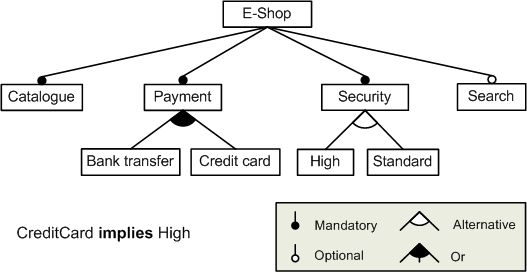
\includegraphics[width=0.7\textwidth]{bilder/E-shopFM.jpg}
\caption{Darstellung eines Featurediagramms für ein konfigurierbares E-Shop System von Segura09 in der Wikipedia auf Englisch (Transferred from en.wikipedia) [Public domain], via Wikimedia Commons}
\label{fig:fd}
\end{figure}

\subsection{Metamodell}

Die Analyse des Problemfelds und Modellierung der Merkmale soll in erster Linie die Grundlage für die Definition des Metamodells der Domäne liefern \cite[S. 200]{stahl2007}. 

\subsubsection{Definition}

Zur Beschreibung welche Mittel zur Definition eines bestimmten Modells zur Verfügung stehen kann man wiederum ein Modell definieren. Dieses, über dem beschriebenen Modell stehende Modell, nennt man Metamodell. Stahl und Voelter bezeichnen es als Beschreibung der möglichen Struktur von Modellen. Dazu zählen sie die Konstrukte der Modellierungssprache, auf welche Weise diese zueinander in Beziehung stehen, sowie vorhandene Regeln bezüglich der Gültigkeit bzw. Modellierung \cite[S. 59]{stahl2007}.

Ein Unified Modeling Language 2.0 (UML) Diagramm welches alle Java Sprachkonzepte, wie beispielsweise die Existenz von Klassen, Attributen und Instanzen, beschreibt, ist eine Darstellung für das Java Metamodell. Geschriebener Java Quelltext wäre somit eine Instanz dieses Modells, kann aber wiederum instanziiert werden. Handelt es sich nämlich um eine Definition einer Java Klasse, so können hiervon Objekte mit konkreten Werten existieren.

Es ist noch hervorzuheben, dass mit dem Begriff Metamodell nicht einfach nur eine Abstraktion gemeint ist. Die Silbe Meta kann hier als  \glqq die Definition von\grqq\ verstanden werden. Ein Modell kann ein anderes Modell abstrahieren in dem es beispielsweise Informationen auslässt, falls diese für ein Anwendungsfall nicht relevant oder implizit sind. Das ist im obigen Sinne dann jedoch noch kein Metamodell. Zu sagen ein Metamodell ist das Modell eines Modells, ist also nur bedingt sinnvoll \cite[S. 27]{voelter2013}.

\subsubsection{Abstrakte Syntax und Konkrete Syntax}

Die in diesem Beispiel definierten Sprachkonzepte sind die abstrakte Syntax für Java. In Abgrenzung hierzu dient eine konkrete Syntax zur Beschreibung eines Modells. Möchte man einen Datentypen definieren, könnte man das mit einem UML Klassendiagramm. Da man den Datentypen auch mit Java-Code beschreiben könnte, sieht man, dass es für dasselbe Metamodell mehr als eine konkrete Syntax geben kann. \cite[S. 59f.]{stahl2007}.

\subsection{Domänenspezifische Sprache (DSL)}

Wurde das Metamodell für eine Domäne definiert, also ist die abstrakte Syntax bekannt, wird eine Möglichkeit benötigt eine Instanz des Metamodells zu bilden. Durch anreichern des Modells mit Informationen wird eine konkrete Ausprägung des Metamodells geschaffen. Das Mittel hierfür ist eine domänenspezifische Programmiersprache.

\subsubsection{Definition}

Stahl und Völter definieren eine solche Programmiersprache mit: \cite[S. 30]{stahl2007}. \glqq Eine DSL ist nichts anderes als eine Programmiersprache für eine Domäne.\grqq Martin Fowler hat in seinem Buch zu diesem Thema eine umfangreichere Definition geschaffen und erläutert diese mit vier Schlüsselelementen \cite[S. 27f.]{fowler2010}.

\begin{quote}\glqq Domain-specific Language (noun): a computer programming language of limited expressiveness focused on a particular domain.\grqq \end{quote}

Der Ausdruck \glqq Computer programming language\grqq\ bedeutet, dass eine DSL vom Menschen verwendet wird um einem Computer Befehle zu geben. Also sollte sie wie jede moderne Programmiersprache durch ihre Struktur sowohl vom Menschen leicht verständlich als auch vom Computer ausführbar sein.

Laut Fowler ist ein weiteres Element die \glqq Language nature\grqq. Als Programmiersprache sollte die Ausdrucksstärke einer DSL nicht nur von den einzelnen Ausdrücke kommen, sondern auch wie die Ausdrücke zusammengesetzt werden.

Mit \glqq Limited expressiveness\grqq\ meint Fowler, dass eine DSL im Vergleich zu allgemeinen Programmiersprachen nur das für die Beschreibung der Domäne notwendige Minimum an Funktionalität aufweist. 

Im letzten Teil seiner Ausführung zu dieser Definition geht Fowler auf den \glqq Domain focus\grqq\ ein. Eine beschränkte Sprache sei nur sinnvoll wenn sie klar auf eine Domäne eingegrenzt ist.

DSLs können in zwei Hauptkategorien unterteilt werden, bezeichnet als interne und externe DSLs.

\subsubsection{General Purpose Language (GPL)}

Die von Fowler angesprochenen allgemeinen Programmiersprachen bezeichnet man als General Purpose Language oder auch abgekürzt als GPL. Im Gegensatz zu DSLs sind GPLs nicht auf eine bestimmte Domäne zugeschnitten, sondern können breiter eingesetzt werden. Moderne Programmiersprachen wie Java und C\# sind solche Universalsprachen. Durch ihre Turing Vollständigkeit, kann man sie untereinander austauschen \cite[S. 111]{hromkovic2014}. Mehr als eine GPL gibt es, da sich einzelne Sprachen durch zusätzliche besondere Sprachfeatures voneinander abheben \cite[S. 27]{voelter2013}. Durch die Unterstützung von Pointern in C ist es zum Beispiel potenziell möglich Datenstrukturen besonders speicheroptimiert anzulegen \cite[S. 93ff.]{kernighan1988}.

\subsubsection{Interne DSLs}

Bettet man die Befehle zur Beschreibung einer Instanz des Metamodells auf geeignete Weise in eine Universalsprache ein, kann man dies interne DSL nennen. Der Aufbau und die Folge von Befehlen soll sich bei einer internen DSL, soweit möglich, wie eine eigene Sprache anfühlen \cite[S 28]{fowler2010}.

Für die Implementation von internen DSLs eignen sich dynamisch zu bezieht Sprachen wie Ruby und Lisp gut, da sie hilfreiche Features wie die Definition von Makros unterstützen. Je mehr in die normale Syntax einer Sprache eingegriffen werden kann, desto eigenständiger lässt sich die Syntax der internen DSL formen \cite[S. 98]{stahl2007}. Hierdurch grenzt sich diese immer weiter von einem einfachen application programming Interface (API) ab. Gerade wenn das Metamodell bei objektorientierter Programmierung in Form von Klassen vorliegt, kann eine interne DSL eher wie eine einfache Schnittstelle wirken. Die Abgrenzung von internal DSL zu API ist nicht eindeutig und stellt eine Grauzone dar \cite[S. 67]{fowler2010}.

Eine erwähnenswerte Sonderform der intern DSLs sind fragmentierte DSLs. Bei diesem Spezialfall wird die Hostsprache, also die Programmiersprache mit der die interne DSL ausgedrückt wird, an einzelnen Stellen mit Informationen angereichert. Reguläre Ausdrücke die als Bruchstücke in einer GPL verwendet werden oder auch Annotationen in Java kann man hier als Beispiel anführen \cite[S. 32]{fowler2010}.

\subsubsection{Externe DSLs}

Eine externe DSL hat genau wie eine GPL eine eigene Syntax, laut Fowler ist es jedoch auch nicht unüblich dass die Syntax einer anderen Sprache, beispielsweise XML,  verwendet wird. Sprachen wie die Structured Query Language (SQL) oder Cascading Style Sheets (CSS) sind externe DSLs \cite[S. 28]{fowler2010}. SQL erlaubt es mit syntaktisch einfachen Mitteln Anfragen an eine Datenbank zu schicken und mit CSS kann die grafische Repräsentation von HTML-Seiten manipuliert werden.

Im Gegensatz zu internen DSLs, welche auf der Struktur der zugrunde liegenden GPL beruhen, erlauben externe DSLs ihre Syntax weitestgehend frei zu gestalten. Für ihre Implementation kann grundsätzlich auf einen reichen Schatz an Techniken, die zum verarbeiten von Programmiersprachen seit Jahren verwendet werden, zugegriffen werden \cite[S. 89]{fowler2010}.

\subsection{Parser}

Ein großer Unterschied zwischen internen und externen DSLs besteht in ihrer Verarbeitung. Während interne DSLs eine Datenstruktur direkt mit Informationen befüllen, muss ein Ausdruck einer externen DSL, genau wie bei einem Ausdruck einer GPL, zuerst auf seinen semantischen Informationsgehalt analysiert werden.

\subsubsection{Einlesen des Quelltextes}

Normalerweise liegt der Quelltext, wie der Name schon sagt, in Textform vor. Wenn im folgenden von Quelltext die Rede ist so ist damit der Source Code von externen DSLs sowie der von GPLs gemeint. 

Zur Verarbeitung liest ein Reader den Quelltext zuerst ein und meist wird dieser dann in einem ersten Schritt zeilenweise von einem Lexer in seine Bestandteile (Token) zerlegt. Diese aufgespaltenen Code Zeilen können dann auf syntaktische Korrektheit geprüft werden und in eine Übergangsrepräsentation überführt werden\cite[S. 29f.]{parr2009}. Eine Form hierfür kann ein Abstract Syntax Tree (AST) sein.

\begin{figure}[htbp]
	\centering
	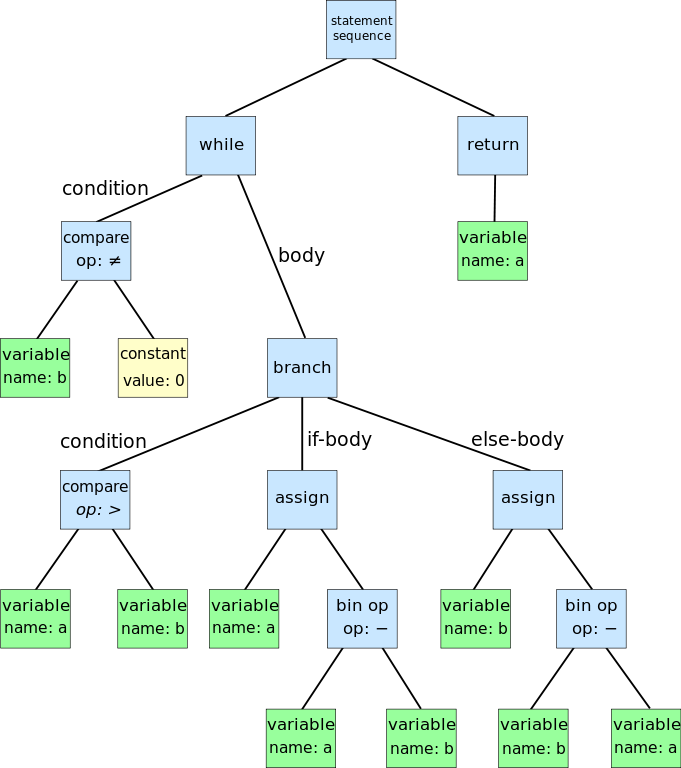
\includegraphics[width=0.7\textwidth]{bilder/euclidean_algorithm_ast}
	\caption{Darstellung des euklidischen Algorithmus als AST von Dcoetzee (Eigenes Werk) [CC0], via Wikimedia Commons}
	\label{fig:ast}
\end{figure}

\subsubsection{Abstract Syntax Tree (AST)}

Für jeden wichtigen Token wird im AST ein Knotenpunkt, mit für den weiteren Prozess wichtigen Daten, angelegt \cite[S. 23]{parr2009}. Die grafische Darstellung  des AST für den euklidischen Algorithmus auf Abbildung \ref{fig:ast} zeigt diese Knoten-basierte Strukturierung des eingelesenen Codes. Die Knoten eines AST kennen ihre eigene Position im Baum und somit kann dieser mit geeigneten Strategien durchlaufen werden \cite[S. 24]{parr2009}.

Eine Möglichkeit ist die Anwendung des Visitor Patterns, welches in dieser Arbeit in einem späteren Unterkapitel der Grundlagen behandelt wird.

\subsubsection{Weitere Verarbeitung des eingelesenen Quelltextes}

Nachdem die syntaktische Korrektheit des Quelltextes sichergestellt ist und dieser in einer geeigneten Datenstruktur vorliegt, stehen jetzt mehrere Möglichkeiten zur Verfügung. Die jetzt in Baumstruktur vorliegenden Anweisungen sind jetzt durch Interpretation von einer Plattform ausführbar. Alternativ könnte auch eine Übersetzung in eine andere Sprache vorgenommen oder direkt zu ausführbaren Maschinencode kompiliert werden.

Bei Java wird der Quelltext beispielsweise eingelesen und zu Byte-Code transformiert, welcher dann von der Java Virtual Machine (JVM) interpretiert werden kann \cite{javavm2014}. Die Übersetzung in eine andere Sprache bietet sich sowohl bei externen DSLs als auch bei GPLs an. Allgemein könnte diese Transformation sinnvoll sein, wenn man seinen Code für eine bestimmte Plattform kompatibel zu einer anderen Plattform machen möchte. Ein Beispiel hierfür ist der Kompilierprozess einer in C\# geschriebenen Unity3D Anwendung zu einer WebGL App. Hierbei wird der C\# Code zuerst in C++ und dann in JavaScript umgewandelt \cite{unity2018}. Native GPLs wie C werden direkt zu Maschinensprache kompiliert \cite{kernighan1988}. Externe DSLs werden von einem Generator häufig zu GPL Quelltext transformiert \cite[S. 26]{voelter2013}.

\subsection{Code Generator}

\subsubsection{Definition}
\subsubsection{Techniken zur Generierung von Code}
\subsubsection{Zusammenhang zu Transformatoren}
\subsubsection{Abgrenzung zum Compilerbau}

\section{Software Architektur}
\subsection{Prinzipien der Softwaretechnik}
\subsubsection{Abstraktion}
\subsubsection{Bindung und Kopplung}
\subsubsection{Modularisierung}
\subsubsection{Weitere Prinzipien}
\subsubsection{Abhängigkeiten}
\subsection{Trennung durch Modelle}
\subsection{Modell-Transformations-Pipeline}

\section{Design Pattern objektorientierter Programmierung}
\subsection{Visitor Pattern}
\subsubsection{Zweck}
\subsubsection{Beschreibung}
\subsubsection{Anwendbarkeit}
\subsection{Builder Pattern und Fluent Interfaces}
\subsubsection{Zweck}
\subsubsection{Beschreibung}
\subsubsection{Anwendbarkeit}
\subsection{Factory Pattern}
\subsubsection{Zweck}
\subsubsection{Beschreibung}
\subsubsection{Anwendbarkeit}

\chapter{Analyse}
\setcounter{section}{-1}
\section[Fragestellung]{Fragestellung: Wie kann, ausgehend von bestehendem Java-Code, ein Meta-Generator zur Erhöhung der Wirtschaftlichkeit Modellgetriebener Softwareentwicklung umgesetzt werden?}
\section{Aufwand eines konventionellen Softwareprojektes im Vergleich zu MDSD}
\section{Automatisierung der Entwicklung eines Code Generators}
\subsection{Java Code als Ausgangsmodell}
\subsubsection{Anreicherung des Java Codes mit Informationen}
\subsubsection{Parsen des Java Codes}
\subsection{Abstrakte Darstellung von Java Code als Modell}
\subsubsection{Anforderungen an das Modell}
\subsubsection{Schnittstellen zur Befüllung des Modells}
(DSLs intern / extern)
\subsection{Generierung von Java Code}
\subsubsection{Techniken zur Code Generierung}
\subsubsection{Vorhandene Frameworks zur Java Code Generierung}

\chapter{Konzept}
\section{Einsparung der Implementation des Code Generators durch einen Meta-Generator}
\section{Funktionsweise des Meta-Generators}
\subsection{Von Java Code zum Annotations-Modell}
\subsubsection{Annotationen als Mittel zur Informationsanreicherung}
\subsubsection{Parsen des annotierten Codes}
\subsubsection{Zweck des Annotations-Modells}
\subsection{Das CodeUnit-Modell}
\subsubsection{Baumstruktur des Modells}
\subsubsection{Spezialisierung durch ein Typ-Feld}
\subsubsection{Parametrisierung durch generische Datenstruktur}
\subsection{Generierung von Buildern als interne DSL aus dem Annotations-Modell}
\subsubsection{Komposition der Builder aus benötigten Builder-Methoden}
\subsubsection{Übertagung vorgegebener Informationen in einen Builder}
\subsubsection{Verwendung von Plattform Code zur Generierung von vordefinierten CodeUnits}
\subsubsection{Auflösung von Referenzen in vordefinierten CodeUnits als nachgelagerter Verarbeitungsschritt}
\subsection{Erzeugung von Java Code aus einem befüllten CodeUnit-Modell}
\subsubsection{Transformation des CodeUnit-Modells zum JavaFile-Modell}
\subsubsection{Erzeugung von Quelldateien}

\chapter{Lösung: Spectrum (Proof of Concept)}
\section{Verwendete Bibliotheken}
\section{Verwendeter Glossar}
\subsection{JavaParser mit JavaSymbolSolver}
\subsection{JavaPoet}
\section{Architekturübersicht}
\subsection{Amber}
\subsubsection{Annotationen}
\subsubsection{Parser}
\subsubsection{Modell}
\subsection{Cherry}
\subsubsection{Generator}
\subsubsection{Modell}
\subsubsection{Plattform}
\subsubsection{Generierte Builder}
\subsection{Jade}
\subsubsection{Transformator}
\subsection{Scarlet}
\subsubsection{Generator}
\subsubsection{Modell}
\subsection{Violet}

\begin{lstlisting}[label=lst:java,
				   language=java,
				   firstnumber=1,
				   caption=Beispiel für einen Quelltext]

public void foo() {
	// Kommentar
}
\end{lstlisting}

\chapter{Evaluierung}
\section{Kozept \& Implementation}
\subsection{Amber}
\subsection{Cherry}
\subsection{Jade}
\subsection{Scarlet}
\section{Softwarequalität}
Nach Balzert S.111
\subsection{Functionality}
\subsection{Maintainability}
\subsection{Performance}
\subsection{Usability}
\section{Grenzen des Lösungsansatzes}

\chapter{Abschluss}
\section{Zusammenfassung}
\section{Ausblick}

\appendix
\chapter{Dokumentation}
\section{Verwendung der Annotationen}
\section{Verwendung der generierten CodeUnit-Builder}
\section{Klassendokumentation}
\subsection{Amber}
\subsection{Cherry}
\subsection{Jade}
\subsection{Scarlet}


\backmatter
%%%%%%%%%%%%%%%%%%%
%% create  list
%%%%%%%%%%%%%%%%%%%

\listoffigures
\addcontentsline{toc}{chapter}{Verzeichnisse}

%%%%%%%%%%%%%%%%%%%
%% create tables list
%%%%%%%%%%%%%%%%%%%
\listoftables

%%%%%%%%%%%%%%%%%%%
%% create listings list
%%%%%%%%%%%%%%%%%%%
%\lstlistoflistings
%\addcontentsline{toc}{chapter}{Listings}

\printbibliography
\addcontentsline{toc}{chapter}{Literatur}

%%%%%%%%%%%%%%%%%%%
%% declaration on oath
%%%%%%%%%%%%%%%%%%%

\addchap{Eidesstattliche Erklärung}

Hiermit versichere ich, dass ich die vorgelegte Bachelorarbeit selbstständig verfasst und noch nicht anderweitig zu Prüfungszwecken vorgelegt habe. Alle benutzten Quellen und Hilfsmittel sind angegeben, wörtliche und sinngemäße Zitate wurden als solche gekennzeichnet.

\vspace{20pt}
\begin{flushright}
$\overline{~~~~~~~~~~~~~~~~~\mbox{\BaAuthor, am \today}~~~~~~~~~~~~~~~~~}$
\end{flushright}

\addchap{Zustimmung zur Plagiatsüberprüfung}

Hiermit willige ich ein, dass zum Zwecke der Überprüfung auf Plagiate meine vorgelegte Arbeit in digitaler Form an PlagScan (www.plagscan.com) übermittelt und diese vorrübergehend (max. 5~Jahre) in der von PlagScan geführten Datenbank gespeichert wird sowie persönliche Daten, die Teil dieser Arbeit sind, dort hinterlegt werden.

\begin{small}
Die Einwilligung ist freiwillig. Ohne diese Einwilligung kann unter Entfernung aller persönlichen Angaben und Wahrung der urheberrechtlichen Vorgaben die Plagiatsüberprüfung nicht verhindert werden. Die Einwilligung zur Speicherung und Verwendung der persönlichen Daten kann jederzeit durch Erklärung gegenüber der Fakultät widerrufen werden.
\end{small}

\vspace{20pt}
\begin{flushright}
$\overline{~~~~~~~~~~~~~~~~~\mbox{\BaAuthor, am \today}~~~~~~~~~~~~~~~~~}$
\end{flushright}

\end{document}
